%% Based on a TeXnicCenter-Template by Gyorgy SZEIDL.
%%%%%%%%%%%%%%%%%%%%%%%%%%%%%%%%%%%%%%%%%%%%%%%%%%%%%%%%%%%%%

%------------------------------------------------------------
%
\documentclass{article}%
%Options -- Point size:  10pt (default), 11pt, 12pt
%        -- Paper size:  letterpaper (default), a4paper, a5paper, b5paper
%                        legalpaper, executivepaper
%        -- Orientation  (portrait is the default)
%                        landscape
%        -- Print size:  oneside (default), twoside
%        -- Quality      final(default), draft
%        -- Title page   notitlepage, titlepage(default)
%        -- Columns      onecolumn(default), twocolumn
%        -- Equation numbering (equation numbers on the right is the default)
%                        leqno
%        -- Displayed equations (centered is the default)
%                        fleqn (equations start at the same distance from the right side)
%        -- Open bibliography style (closed is the default)
%                        openbib
% For instance the command
%           \documentclass[a4paper,12pt,leqno]{article}
% ensures that the paper size is a4, the fonts are typeset at the size 12p
% and the equation numbers are on the left side
%
\usepackage{amsmath}%
\usepackage{amsfonts}%
\usepackage{amssymb}%
%--------Graphics Packages------------------
\usepackage{graphicx}
%-------------------------------------------
\newtheorem{theorem}{Theorem}
\newtheorem{acknowledgement}[theorem]{Acknowledgement}
\newtheorem{algorithm}[theorem]{Algorithm}
\newtheorem{axiom}[theorem]{Axiom}
\newtheorem{case}[theorem]{Case}
\newtheorem{claim}[theorem]{Claim}
\newtheorem{conclusion}[theorem]{Conclusion}
\newtheorem{condition}[theorem]{Condition}
\newtheorem{conjecture}[theorem]{Conjecture}
\newtheorem{corollary}[theorem]{Corollary}
\newtheorem{criterion}[theorem]{Criterion}
\newtheorem{definition}[theorem]{Definition}
\newtheorem{example}[theorem]{Example}
\newtheorem{exercise}[theorem]{Exercise}
\newtheorem{lemma}[theorem]{Lemma}
\newtheorem{notation}[theorem]{Notation}
\newtheorem{problem}[theorem]{Problem}
\newtheorem{proposition}[theorem]{Proposition}
\newtheorem{remark}[theorem]{Remark}
\newtheorem{solution}[theorem]{Solution}
\newtheorem{summary}[theorem]{Summary}
\newenvironment{proof}[1][Proof]{\textbf{#1.} }{\ \rule{0.5em}{0.5em}}

\begin{document}

\begin{flushleft}
\textbf{Course:} CSC707, Automata, Computability and Computational Theory\\
\textbf{Homework 4}: Finite automata (FA), DFA, NFA, regular expressions, Pumping lemma, and closure properties\\
\textbf{Submission:} Use Wolfware\\
\textbf{File Format:} LaTeX and PDF\\
\textbf{NOTE:} If you create images, make sure you submit them as well.
\end{flushleft}

\begin{center}
\fbox{\textbf{Due Date:} \textbf{11:00 AM, Saturday, March 13, 2010}}\\
\end{center}

\noindent{\hrulefill}

\bigskip

\begin{enumerate}

	\item Given the set of all of strings in $(0+1)^*$ such that some two zeros are separated by a string whose length is $4i$, for some some $i \geq 0$,
		\begin{enumerate}
		\item Give a nondeterministic finite automata accepting this set.
		\item Provide a regular expression for $L$.
	\end{enumerate}
	
\textbf{Answer:}
\begin{enumerate}
	\item 
		\begin{figure}[h]
\centering
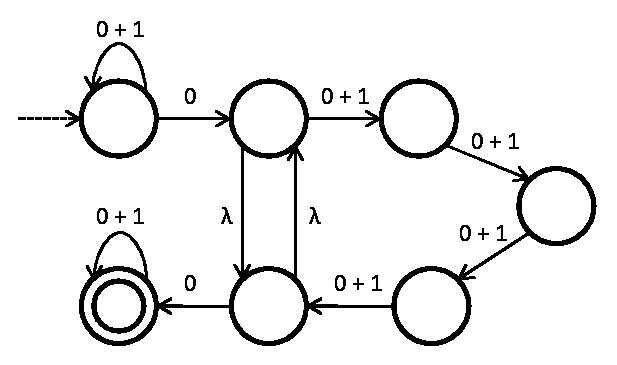
\includegraphics[scale=0.8,clip]{nfa.eps} 
\end{figure}
	\item The regular expression for $L$ is: $$(0+1)^*0((0+1)(0+1)(0+1)(0+1))^*0(0+1)^*$$ 
	
%	The regular expression for $L$ is: $$1^* (01111(1111)^* + 001111(1111)^*)^*(\lambda+0+00) 1^*$$
\end{enumerate}


	\item Given a language $L$ of all strings over $\{0,1\}$ with an equal number of zeros and ones such that no prefix has two more zeros than ones nor has two more ones than zeros:	
	\begin{enumerate}
		\item  Construct a DFA that accepts all strings from $L$.
		\item  Provide a regular expression for $L$.
	\end{enumerate}

\textbf{Answer:}
\begin{enumerate}
	\item 
	
	\begin{figure}[h]
\centering
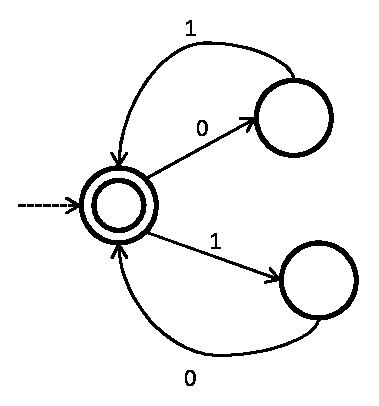
\includegraphics[scale=0.8,clip]{dfa.eps} 
\end{figure}
	\item The regular expression for $L$ is: $(01+10)^*$
\end{enumerate}


	\item Which of the following languages are regular? Prove your answers.	
	\begin{enumerate}
		\item  $L = \{ 0^j |{\rm{ }}j\bmod 3 \equiv 0\}$
		\item  $L = \{ 0^j 1^k |{\rm{ gcd(}}j,k) \equiv 1\}$, where $gcd()$ is the greatest common denominator.
		\item  $L = \{ 0^i 1^j 0^k |{\rm{ }}k \ge i + j\} $
	\end{enumerate}
	
	
\begin{enumerate}
	\item 
	\begin{theorem}
	$L = \{ 0^j |{\rm{ }}j\bmod 3 \equiv 0\}$ is regular language.
	\end{theorem}
	
	\begin{proof}
	Language $L$ accepts strings formed by 0s whose number is the multiple of 3. We can use the regular expression $(000)^*$ to accept $L$.
	\end{proof}
	
		\item 
	\begin{theorem}
	$L = \{ 0^j 1^k |{\rm{ gcd(}}j,k) \equiv 1\}$ is not regular language.
	\end{theorem}
	
	\begin{proof}
	We can use pumping lemma to prove it.
	Assume that $L$ is regular. Let $p$ be the pumping length and $x$ is the product of the primes $\leq p + 1$. For two integer $j,k$, if $gcd(j,k)=1$, they are relatively prime. Since any two consecutive integers are relatively prime, we can pick $s=0^{x+1}1^{x}$. From the pumping lemma, we can write $s=xyz$ such that $|xy| \leq p$. Thus, $y$ must be $0^{m}$, where $1 \leq m \leq p$. Now we consider $s' = xy^{i}z$ and $i = 2$. From $y=0^{m}$, we can have $s'=0^{x+1+m}1^{x}$. Since $1 \leq m \leq p \Rightarrow 2 \leq m + 1 \leq p+1$, all the prime factors of $m+1$ are $\leq p + 1$ (if $m+1$ is prime, then the prime factor of $m+1$ is itself). Since $x$ is the product of the primes $\leq p + 1$, the prime factors in $m+1$ must be in $x$. Thus, there exists a common factor $f$ between $x$ and $m+1$, which shows that $x+1+m$ has a common factor with $x$. Hence, $s' \notin L$. By pumping lemma, $L$ is not regular language.	
	
	\end{proof}
	
		\item 
	\begin{theorem}
	$L = \{ 0^i 1^j 0^k |{\rm{ }}k \ge i + j\} $ is not regular language.
	\end{theorem}
	
	\begin{proof}
	We can use pumping lemma to prove it.
	Assume that $L$ is regular. Let $p$ be the pumping length. We can pick $s=o^p1^p0^{2p}$, which is in $L$. From the pumping lemma, we can write $s=xyz$ such that $|xy| \leq p$. Thus, $y$ must be $0^{m}$, where $1 \leq m \leq p$. Now we consider $s' = xy^{a}z$ and $a = 2$. From $y=0^{m}$, we can have $s'=0^{p+m}1^{p}0^{2p}$. In $s'$, $i=p+m$,$j=p$, and $k=2p$. Since $i+j=2p+m$ and $1 \leq m \leq p$, $2p+m \ge 2p = k$. Thus, $s' \notin L$. By pumping lemma, $L$ is not regular language.	
	\end{proof}
	
	\end{enumerate}
%----------------------------------------------------------------------------
	\item Assuming $L_1 ,L_2 ,...$ are regular, which of the following languages are regular. Prove your answers.	
	\begin{enumerate}
		\item  $\bigcup\limits_{i = 1}^n {L_i } $
		\item  $\bigcup\limits_{i = 1}^\infty  {L_i } $
	  \item  $\bigcap\limits_{i = 1}^n {L_i } $
		\item  $\bigcap\limits_{i = 1}^\infty  {L_i } $
	\end{enumerate}

%----------------------------------------------------------------------------

	\item Prove that the following languages are regular:
	\begin{enumerate}
	\item  $MIN(L) = \{ x \in L |$ no prefix of $x$ is in $L$\}
	\item  $L^R  = \{ x|$ reverse of $x$ is in $L\}$
	\end{enumerate}

	
\end{enumerate}

\end{document}
